\subsection*{3.1 Components used}

This project consists of both hardware and software components. The hardware components used in this project are discussed below:

\subsubsection*{3.1.1 Johnson motor}

A Johnson motor is a brushed DC motor that contains permanent magnets. It is a high-speed motor with high torque and widely used in robotic applications. In this project, Johnson motors are used for driving the wheels of the robot.

\begin{figure}[H]
    \centering
    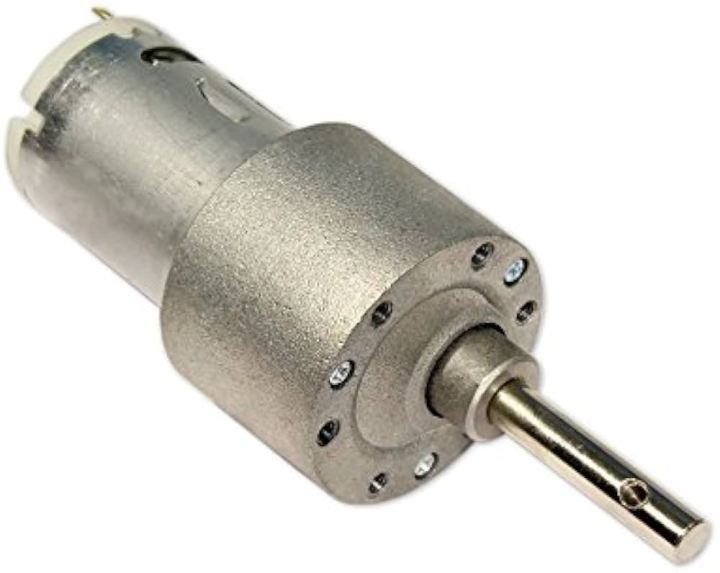
\includegraphics[width=0.5\textwidth]{3.1.jpg}
    \caption{\textbf{Johnson Motor[https://www.daraz.com.np/products/johnson-motor-metal-gear-300rpm-i129797381.html]}}
    \label{fig:3.1}
\end{figure}

\subsubsection*{3.1.2 Raspberry Pi 4}

Raspberry Pi 4 is a credit card-sized computer that can run an operating system and perform multiple functions. It is equipped with a Broadcom BCM2711, Quad core Cortex-A72 (ARM v8) 64-bit SoC @ 1.5GHz, 2GB RAM, and USB and HDMI ports. In this project, it processes voice commands, sends control signals to Arduino, and communicates with cloud services.

\begin{figure}[H]
    \centering
    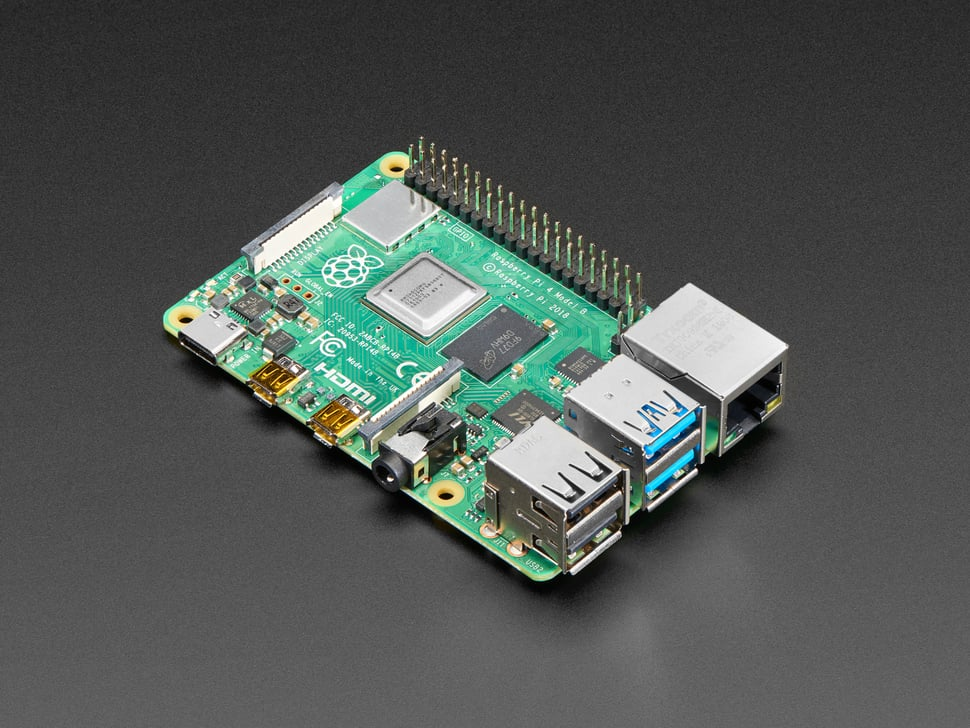
\includegraphics[width=0.5\textwidth]{fig3.2.jpg}
    \caption{\textbf{Raspberry Pi 4[https://www.adafruit.com/product/4292]}}
    \label{fig:3.2}
\end{figure}

\subsubsection*{3.1.3 Arduino UNO}

The Arduino UNO is an open-source microcontroller board based on the Microchip ATmega328P microcontroller. It features 14 digital I/O pins, 6 analog inputs, a 16 MHz quartz crystal, and USB and power jack. In this project, it controls motors and sensors based on the instructions received from the Raspberry Pi.

\begin{figure}[H]
    \centering
    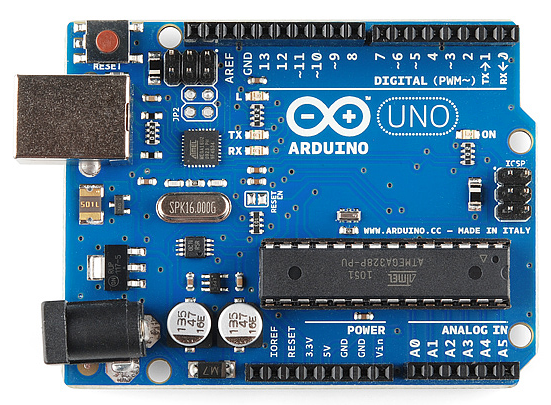
\includegraphics[width=0.5\textwidth]{fig3.3.png}
    \caption{\textbf{Arduino UNO[https://digilog.pk/products/arduino-uno-kit-in-pakistan]}}
    \label{fig:3.3}
\end{figure}

\subsubsection*{3.1.4 IR Array Sensor}

IR (Infrared) array sensors are used to detect the path for line-following by emitting and detecting IR light. A group of IR sensors is arranged to detect black lines on a white surface. In this project, they help the robot follow the designated path.

\begin{figure}[H]
    \centering
    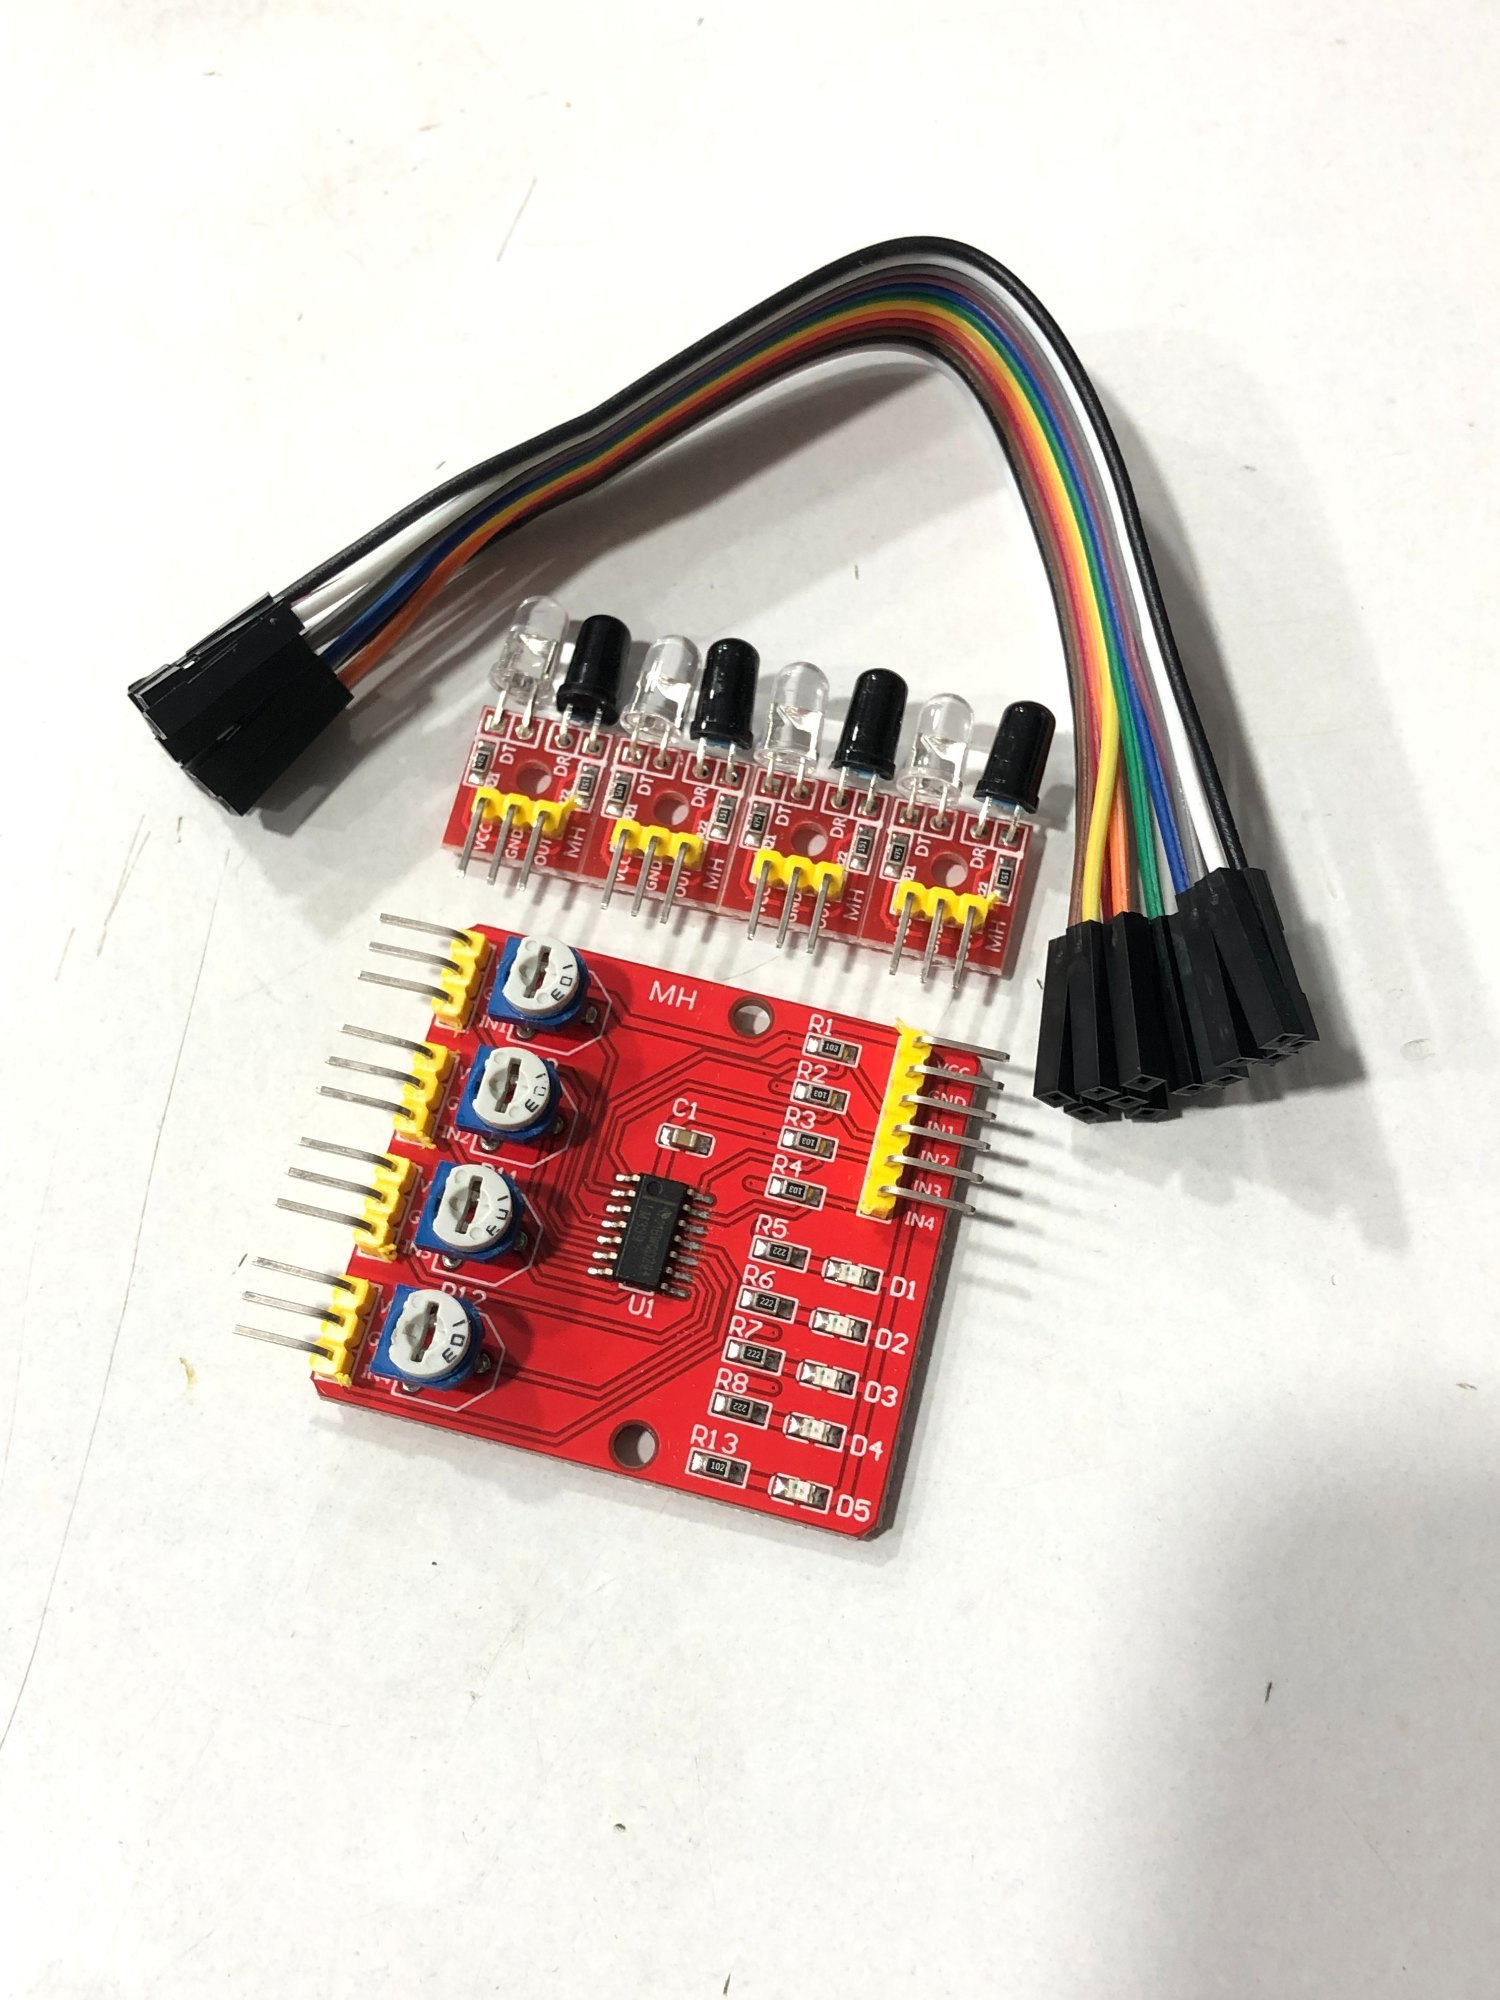
\includegraphics[width=0.5\textwidth]{3.4.jpg}
    \caption{\textbf{IR Array Sensor[https://www.giganepal.com/product/ir-sensor-array-module-4-way/?v=584a79c5e916]}}
    \label{fig:3.4}
\end{figure}

\subsubsection*{3.1.5 Metal Gear Servo MG996R}

The MG996R is a high-torque servo motor with metal gears and digital control. It provides accurate angle control and is used in the pill dispensing mechanism. It can rotate 0–180 degrees and is known for durability and stability.

\begin{figure}[H]
    \centering
    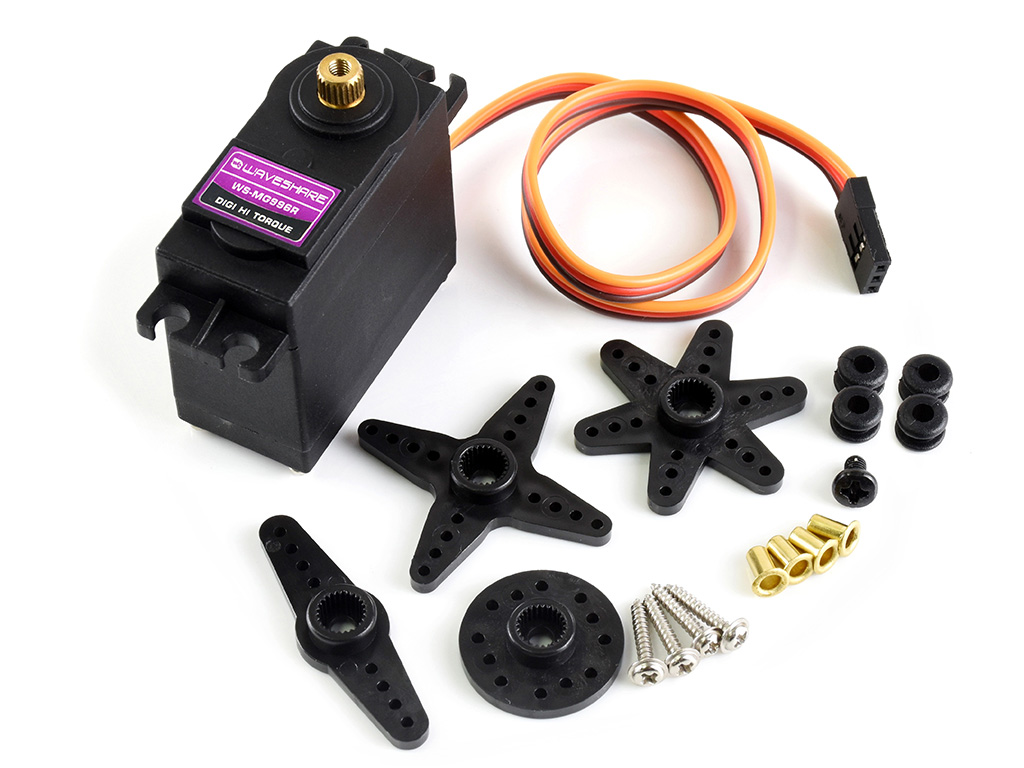
\includegraphics[width=0.5\textwidth]{3.5.jpg}
    \caption{\textbf{Metal Gear Servo MG996R[https://www.waveshare.com/mg996r-servo.htm]}}
    \label{fig:3.5}
\end{figure}

\section{Software}

\textbf{Arduino IDE:} The Arduino Integrated Development Environment (IDE) is used to program the Arduino microcontroller responsible for real-time control of motors, sensors, and actuators. Written in C/C++, the code implements PID algorithms for accurate line following, triggers pill dispensing via servo motors, and reads data from modules such as IR sensors, UHF RFID readers, and ultrasonic sensors. Libraries like \texttt{Servo.h}, \texttt{Wire.h}, and \texttt{SoftwareSerial.h} simplify hardware interactions. Serial communication with the Raspberry Pi enables synchronous operation and system-level decision-making. The IDE’s Serial Monitor is invaluable for debugging sensor readings and validating motor responses, supporting firmware-level coordination for the robot’s motion and dispensing tasks.

\vspace{0.5em}

\textbf{Raspberry Pi \& Camera Module:} The Raspberry Pi 4 Model B, paired with the Raspberry Pi Camera V2 (NoIR), serves as the high-level processing unit of the system. It runs Python scripts for facial recognition using OpenCV and manages scheduled pill dispensing through a timetable system. Sensor feedback and motor status are received from the Arduino via UART serial communication, enabling dynamic coordination based on environmental inputs and patient recognition. The onboard real-time clock (RTC, optional) ensures precise execution of time-based actions. Captured facial data is matched with a patient database to ensure accurate medication delivery. A local SQLite or CSV-based logging system maintains records for real-time auditing and system monitoring.

\vspace{0.5em}

\textbf{Blender:} Blender, while not central in the current phase, may be employed for visual prototyping, robot path planning simulation, and 3D modeling of the robot’s compartments—including sliding tray mechanisms and modular structures. Using Blender’s Python API (\texttt{bpy}), simulations of compartment stacking and CAD-like assemblies can be rendered, providing a clear indication of hardware integration points and assisting in early-stage design validation.

\vspace{0.5em}

\textbf{Python Middleware:} Python acts as a critical middleware layer, bridging hardware and software. With \texttt{PySerial}, it decodes raw Arduino sensor data (e.g., accelerometer, gyroscope) into actionable gesture commands. These commands can trigger Blender animations via the \texttt{bpy} API, mapping real-world motions to virtual actions like grabbing or rotating objects. Python scripts also handle sensor calibration, noise filtering, and data normalization, enhancing interaction accuracy. This versatile setup supports rapid prototyping—from adjusting sensor thresholds to automating simulation updates—ensuring seamless real-time communication between hardware and virtual environments.



%\section{Dataset}
%\lipsum[4-8]
